\section{Introduction}

% 这部分主要要求将动机

% 第一段，直接引出 IKGQA 问题
% 跳过 LLM 的介绍，直接写 KGQA 再到 IKGQA
% Benefiting from large parameter scales and extensive training data, Large Language Models (LLMs) have achieved impressive results across various tasks, including text generation~\cite{li2023deliberate, tan2024proxyqa}, question answering~\cite{wang2024t, li2024unigen, zong2024triad}, and translation~\cite{brown2020language, zhu2023multilingual, man2025dmdteval}. However, LLMs often generate factually incorrect but plausible responses, known as hallucinations. To address this issue, recent studies introduce external knowledge graphs (KGs) as structured and semantically rich sources of information to enhance the factual reliability of LLM-generated responses~\cite{luo2023reasoning, chen2024plan, tan2025paths, ma2025debate}. 


Recent advances in Knowledge Graph-based Question Answering (KGQA) have shown that augmenting larges language models (LLMs) with structured, semantically rich knowledge graphs (KGs) can improve the factual reliability of model outputs~\cite{luo2024reasoning, chen2024plan, tan2025paths, ma2025debate}. These methods typically retrieve KG subgraphs relevant to the input query and feed them into the LLM in a multi-step manner, thereby improving answer quality~\cite{sun2023think}. Although effective, these methods tend to rely on the completeness of the underlying knowledge graphs—conditions that are difficult to satisfy in practice due to the high cost of KG construction and maintenance~\cite{hur2021survey}. Previous studies have recognized the challenge of KG incompleteness~\cite{min2013distant, ren2020query2box, pflueger2022gnnq}, which has led to the emergence of \textbf{Incomplete Knowledge Graph Question Answering (IKGQA)} as a distinct research task. 

% zan2022complex, zhao2022improving, 
To address the IKGQA issue, existing approaches can be broadly categorized to: (i) KG-internal completion, and (ii) external information augmentation. For category (i), KG-internal completion methods typically aim to predict missing links by learning embedding representations of entities and relations, modeling relational patterns among existing triples within the KG~\cite{saxena2022sequence, guo2023knowledge}. However, such methods inherently rely on existing KG structure and thus struggle to capture changes in the external world, as real-world KG incompleteness often arises from evolving events. Category (ii) includes methods that mitigate KG incompleteness by incorporating knowledge sources beyond the KG itself. some approaches leverage external textual corpora, such as Wikipedia, to construct question-specific subgraphs and enrich the KG with supplementary contextual information~\cite{sun2019pullnet, lv2020graph}. Others treat the parametric knowledge embedded in LLMs as an auxiliary information source, using it to infer missing triples~\cite{xu2024generate}. While these methods demonstrate the value of incorporating external information to mitigate KG incompleteness, they still exhibit notable limitations. Approaches that integrate structured and unstructured data typically rely on training models with substantial amounts of aligned data, making them sensitive to the quality and coverage of training resources. On the other hand, methods that rely exclusively on the parametric knowledge encoded in LLMs may yield incorrect inferences when the missing KG facts fall beyond the coverage of the LLMs' pre-training. These limitations raise a central question: How to leverage inference capabilities of LLM to better integrate mixed knowledge for the IKGQA issue?

\begin{figure}[t]
    \centering
    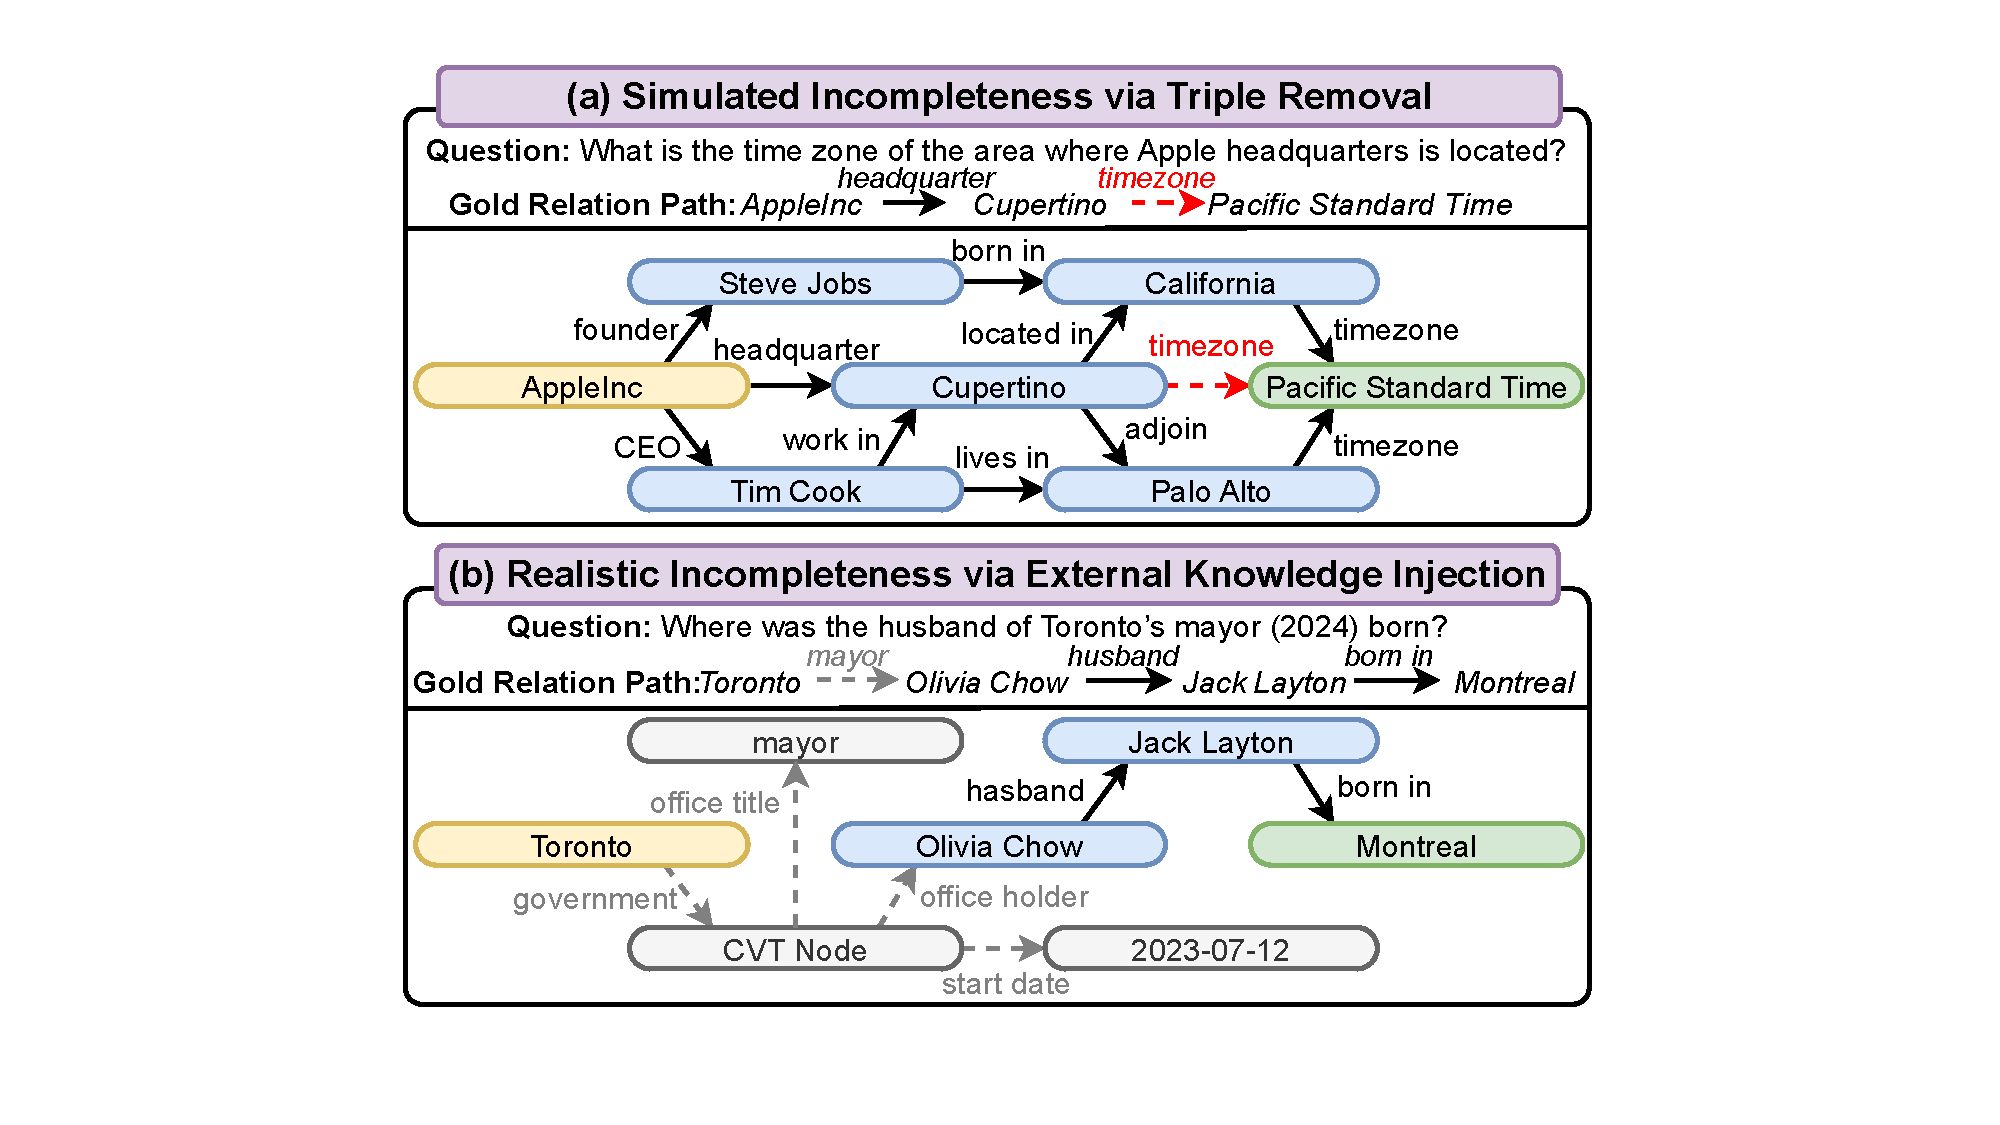
\includegraphics[width=\linewidth]{figures/figure_0.pdf}
    \caption{Illustration of two strategies for constructing incomplete KG scenarios. (a) Simulated incompleteness by removing triples from the KG; red dashed arrows denote the deleted facts. (b) Realistic incompleteness by incorporating external knowledge; gray dashed arrows indicate newly introduced information. CVT (Compound Value Type) nodes are used to represent multi-entity relations in Freebase.}
    \label{fig:IKG_Construction}
\end{figure}

To this end, we propose Debate over Mixed-knowledge (DoM). Given the need to effectively integrate external and KG-based knowledge, we adopt the Multi-Agent Debate (MAD) framework, where independent agents specialize in performing inference over different knowledge sources and collaboratively refine their outputs through interaction and alignment. Specifically, to effectively combine MAD with IKGQA, we introduce a three-stage framework : (1) Initialization: to prepare for effective coordination of mixed-knowledge, we decompose the input question into semantically coherent sub-questions. These sub-questions are dynamically updated throughout the inference process. (2) Sub-question Inference: to integrate heterogeneous knowledge, we design dual retrieval agents, including a KG Agent for structured KG and a Retrieval-Augmented Generation (RAG) Agent for unstructured external knowledge. Each agent independently retrieves candidate evidence, and a Judge Agent evaluates and integrates their outputs to produce an intermediate answer and update the inference plan. This design enables mutual correction and complementarity between knowledge sources. (3) Final Answer Generation: to ensure global consistency, DoM prompts an LLM to consolidate intermediate results into a final answer. However, existing IKGQA datasets typically simulate incompleteness by randomly removing gold-path triples. This synthetic pattern fails to capture the irregular and evolving nature of real-world incomplete KG scenarios. To address this limitation, we construct a new dataset, Incomplete Knowledge Graph WebQuestions (IKGWQ), by revisiting existing QA benchmarks (CWQ and WebQSP) and regenerating question-answer pairs using up-to-date knowledge. This design naturally introduces both missing triples and missing entities, thereby capturing the evolving nature of real-world KG incompleteness.
Finally, extensive experiments demonstrate the effectiveness of our proposed \shortname. Our main contributions are summarized as follows:


% However, existing IKGQA datasets typically simulate incompleteness by randomly removing gold-path triples. This synthetic pattern fails to capture the irregular and evolving nature of real-world incomplete KG scenarios. To address this limitation, we construct a new dataset, Incomplete Knowledge Graph WebQuestions (IKGWQ), by revisiting existing QA benchmarks (CWQ and WebQSP) and regenerating question-answer pairs using up-to-date knowledge. This design naturally introduces both missing triples and missing entities, thereby capturing the evolving nature of real-world KG incompleteness.


\begin{enumerate}
    \item To better integrate multi-source knowledge to address the IKGQA challenge, we propose a multi-agent debate framework, Debate over Mixed-knowledge (DoM), which enables dynamic and complementary inference from incomplete KGs and external knowledge.
    % \item Experimental results show that DoM outperforms the strongest existing baseline by up to 13.6\% under different evaluation settings on existing IKGQA datasets.
    % \item We construct a new dataset, Incomplete Knowledge Graph WebQuestions (IKGWQ), which more accurately reflects real-world KG incompleteness by introducing evolving events that extend beyond the knowledge in the KG. DoM also achieves state-of-the-art performance on IKGWQ, surpassing the best baseline by 70.7\%.
    \item We construct a new dataset, IKGWQ, addressing the limitations of existing IKGQA datasets by introducing real-world factual updates, better reflecting the irregularity and unpredictability of KG incompleteness.
    \item DoM achieves consistent gains over strong baselines, with up to 13.6\% relative improvement in Hits@1 on existing IKGQA datasets and 70.7\% on IKGWQ.
\end{enumerate}



